% !TeX spellcheck = fr_FR

% TODO: Replace scan images with clean text where possible

\documentclass[a4paper, 10pt]{report}

\usepackage[french]{babel}
\usepackage[T1]{fontenc}

\usepackage{amsmath, amssymb, amsfonts}

\usepackage{hyperref}
\usepackage{geometry}

\usepackage{xcolor}
\usepackage{graphicx}

\usepackage{fancyhdr}
\usepackage{lastpage}

\usepackage{enumitem}

\geometry{
	a4paper,
	left=25mm,
	right=25mm,
	top=35mm,
	bottom=25mm,
	headsep=5mm,
	headheight=20mm,
}

\definecolor{solution}{HTML}{E5E4E2}
\providecommand{\abs}[1]{\lvert#1\rvert}
\providecommand{\norm}[1]{\lVert#1\rVert}

\begin{document}
	
	\renewcommand{\headrule}{%
		\vspace{-4pt}\hrulefill
		\raisebox{-6.8pt}{\ 
\includegraphics[height=5mm]{../../icon.png}}
		\hrulefill
	}	
	\pagestyle{fancy}
	\fancyhf{}
	
	\fancyhead[L]{\small \slshape Automne 2024}
	\fancyhead[C]{\Large \bfseries Logique et Théorie des Ensembles\\
		Série 02-B}
	\fancyhead[R]{\small Buff Mathias}
	\fancyfoot[L]{
		\small Source files available at:
		\href{https://github.com/MathiasBuff/bsc-math}
		{github.com/MathiasBuff/bsc-math}
	}
	\fancyfoot[R]{
		\small Page \thepage
		\hspace{1pt} /
		\pageref*{LastPage}
	}
	
	\noindent
	\textbf{Exercice 1.} En partant de l'ensemble vide, construire à
	l'aide des axiomes des ensembles à $10$ et $2^{10}$ éléments.
	Pensez-vous pouvoir construire des ensembles de taille finie
	quelconque ?
		
	\colorbox{solution}
	{
		\begin{minipage}{0.9\textwidth}
			Partons de $\emptyset$ : 0 élément.\\
			Par l'axiome de puissance,
			\[\begin{aligned}
				&\mathcal{P}(\emptyset) = \{\emptyset\}
					\ \text{: 1 élément}\\
				&A = \mathcal{P}(\mathcal{P}(\emptyset)) =
					\{\emptyset, \{\emptyset\}\} \ \text{: 2 éléments}\\
				&B = \mathcal{P}(A) =
					\{\emptyset, \{\emptyset\}, \{\{\emptyset\}\},
					\{\emptyset, \{\emptyset\}\}\}
					\ \text{: 4 éléments}\\
			\end{aligned}\]
			Par l'axiome de compréhension,
			\[
				C = \Bigg\{x \in \mathcal{P}(B)\ \text{tel que}\
					x \notin B \ \text{et} \ x \notin
					\bigg\{
					\Big\{\emptyset, \{\{\emptyset\}\}\Big\},
					\Big\{\{\emptyset\}, \{\{\emptyset\}\}\Big\}
					\bigg\}
				\Bigg\}
			\]
			
			$C$ possède alors $2^4 - 4 - 2 = 10$ éléments, et donc
			$\mathcal{P}(C)$ possède $2^{10}$ éléments.
			
			\vspace{5mm}
			On peut remarquer que l'axiome de puissance permet de
			construire des ensembles de grande taille, et l'axiome
			de compréhension permet de restreindre librement le
			nombre d'éléments d'un ensemble. On en déduit donc qu'il
			est possible de construire des ensembles de taille finie
			quelconque.
		\end{minipage}
	}
	
	\newpage
	
	\fancyhf{}
	\renewcommand{\headrule}
	{\rule{\textwidth}{0pt}}
	\fancyfoot[R]{
		\small Page \thepage
		\hspace{1pt} /
		\pageref*{LastPage}
	}
	
	\noindent
	\textbf{Exercice 2.} (Différence symétrique). L'opération
	$\bigtriangleup$ est définie sur les ensembles $A, B \subset E$\\
	par $A \bigtriangleup B =
		(A \cap (E \setminus B)) \cup (B \cap (E \setminus A))$.
	
	\begin{enumerate}[label=\arabic*.]
		\item Montrer que : $A \bigtriangleup B =
			(A \cup B) \setminus (A \cap B)$.
		%
		\item Vérifier que : $A \bigtriangleup B = \emptyset
			\iff (A = B)$.
	\end{enumerate}
	
	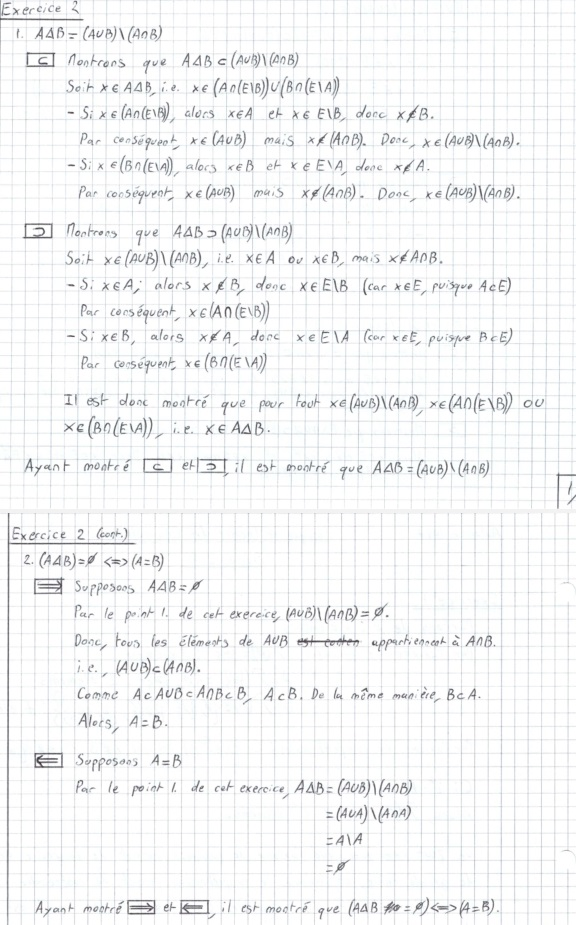
\includegraphics[scale=0.8]{02B - ex02.jpg}
	
	\newpage

	\noindent
	\textbf{Exercice 3.} Soient $E, F$, et $G$ trois ensembles.
	
	\begin{enumerate}[label=\arabic*.]
		\item Montrer que $E \cup (F \cap G)
			= (E \cup F) \cap (E \cup G)$.
		%
		\item Montrer que $E \setminus (F \cup G)
			= (E \setminus F) \cap (E \setminus G)$.
		%
		\item Montrer que $E \setminus (F \cap G)
		= (E \setminus F) \cup (E \setminus G)$.
	\end{enumerate}
	
	
	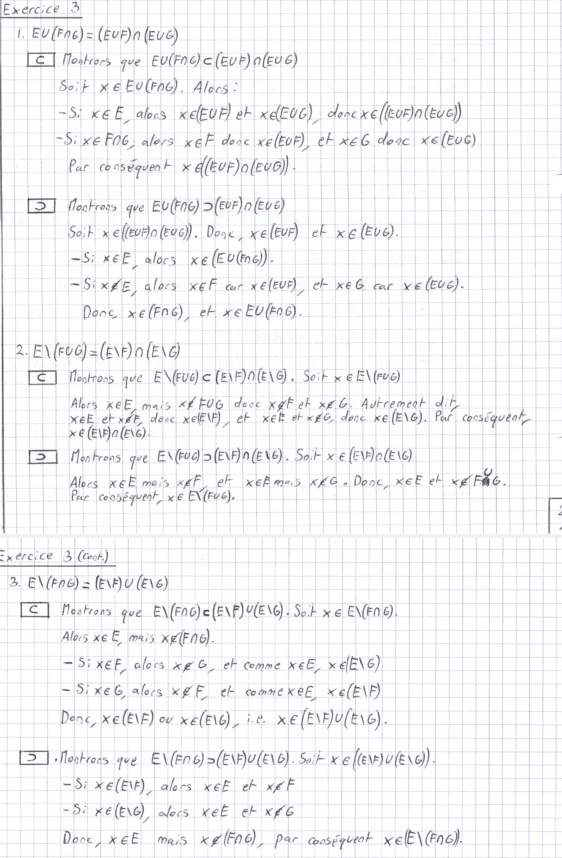
\includegraphics[scale=0.9]{02B - ex03.jpg}
	
	\newpage
	
	\noindent
	\textbf{Exercice 4.} Montrer que $E = F$ si et seulement si
	$\mathcal{P}(E) = \mathcal{P}(F)$.
	
	\colorbox{solution}
	{
		\begin{minipage}{0.9\textwidth}
			Montrons $E = F \iff \mathcal{P}(E) = \mathcal{P}(F)$.
			Raisonnement par double implication :
			\begin{itemize}
				\item[\fbox{\parbox[t][0pt]{6mm}{$\implies$}}]
				Supposons $E = F$.\\
				En particulier, $E \subset F$ donc toute partie de $E$
				est également partie de $F$.\\
				Donc, $\mathcal{P}(E) \subset \mathcal{P}(F)$.
				
				Par le même raisonnement, puisque $F \subset E$ alors
				$\mathcal{P}(F) \subset \mathcal{P}(E)$.
				
				Comme $\mathcal{P}(E) \subset \mathcal{P}(F)$ et
				$\mathcal{P}(F) \subset \mathcal{P}(E)$, alors
				$\mathcal{P}(E) = \mathcal{P}(F)$
				
				\vspace{5mm}
				
				\item[\fbox{\parbox[t][0pt]{6mm}{$\impliedby$}}]
				Supposons $\mathcal{P}(E) = \mathcal{P}(F)$.\\
				Soit $A$ une partie de $E$. Comme $A \subset E$,
				alors $A \in \mathcal{P}(E)$ et puisque
				$\mathcal{P}(E) = \mathcal{P}(F)$, alors
				$A \in \mathcal{P}(E)$ et donc $A \subset F$.			
				Puisque $A$ est générale, $E \subset F$.
				
				De la même manière, il peut être montré que
				$F \subset E$.\\
				Comme $E \subset F$ et $F \subset E$, $E = F$.
			\end{itemize}
			
		\end{minipage}
	}
	
	\vspace{5mm}
	\noindent
	\textbf{Exercice 5.} Expliciter les éléments de l'ensemble
	$\mathcal{P}(\mathcal{P}(\{0\}))$.
		
	\colorbox{solution}
	{
		\begin{minipage}{0.9\textwidth}
			Les éléments de $\{0\}$ sont : $0$\\
			Les éléments de $\mathcal{P}(\{0\})$ sont : $\emptyset, \{0\}$\\
			Les éléments de $\mathcal{P}(\mathcal{P}(\{0\}))
				= (\mathcal{P}(\{\emptyset, \{0\}\})$ sont :
				$\emptyset, \{\emptyset\}, \{\{0\}\}, \{\emptyset, \{0\}\}$\\
			
			Donc, $\mathcal{P}(\mathcal{P}(\{0\})) =
			\{\emptyset, \{\emptyset\}, \{\{0\}\}, \{\emptyset, \{0\}\}\}$
		\end{minipage}
	}
	
	\vspace{5mm}
	\noindent
	{\color{red}\textbf{Exercice 6.}}
	Montrer qu'il n'existe pas d'ensemble $F$ de tous les ensembles
	(on pourra raisonner par l'absurde et considérer la partie de $F$
	composée des ensembles ne s'appartenant pas).
		
	\colorbox{solution}
	{
		\begin{minipage}{0.9\textwidth}
			\textbf{Preuve par l'absurde :}\\
			Supposons $F$ l'ensemble de tous les ensembles, et $A$ la
			partie de $F$ composée des ensembles ne s'appartenant pas.
			
			Si $A$ s'appartient, alors $A$ n'est pas un élément de $A$,
			donc $A$ ne s'appartient pas, et par conséquent $A$ est
			un élément de $A$, donc $A$ s'appartient.
			
			Cette situation mène donc à un paradoxe, et on peut en
			déduire que l'ensemble de tous les ensembles ne peut pas
			exister.
		\end{minipage}
	}
	
\end{document}
